\chapter{Pressure, Equation of State, and Vacuum Energy}

This lecture begins in question-and-answer mode and only gradually becomes a derivation. We first clear away conceptual confusion about the cosmic microwave background, preferred frames, superluminal recession, and horizons. Only then do we turn to the real technical target: the relation between pressure and energy density, the equation-of-state parameter \(w\), and the special role of vacuum energy. The present companion notes follow Leonard Susskind's order closely, preserve the relevant board evidence, and acknowledge Leonard Susskind, LazyingArt LLC, and Video2Book.

\section{Opening Questions: Preferred Frame, Recession, and the CMB}

The first question is about the microwave background: if the cosmic radiation looks isotropic only in one frame, does that not define a preferred frame of reference? Susskind's answer is yes, it does, and that is not a contradiction of relativity. The preferred frame is simply the frame in which the microwave background is isotropic. It is also, on average, the frame in which the nearby galaxies are at rest.

If we move through the microwave background, then the Doppler effect makes photons in the direction of motion appear bluer and photons in the opposite direction appear redder. The isotropy is therefore spoiled by our motion. This is not a failure of relativity. It is a statement about the state of the universe, not about a breakdown of the local laws of physics.

The next question asks whether distant galaxies can recede faster than light. Here the correct distinction is between local relative motion and cosmological recession. Locally, no observer sees a nearby object pass with speed greater than \(c\). Globally, however, the Hubble law can assign recession speed greater than \(c\) to sufficiently distant galaxies:
\begin{equation}
v = H d .
\end{equation}
If \(d\) is large enough, then \(v\) can exceed \(c\). In the units used throughout the lecture we set \(c=1\), so the horizon is the place where \(Hd=1\).

This also clarifies the relation between the cosmic horizon and the surface of last scattering. They are not exactly the same thing. The horizon is the place from which light would arrive only with infinite redshift. The surface of last scattering is slightly inside that limit. We do see it, but only after a large redshift, of order \(10^3\). For many purposes it lies very near the horizon, but conceptually it is not identical to it.

\section{Expanding Metric and the One-Dimensional Line Analogy}

Susskind then shifts from special-relativistic intuition to general-relativistic intuition. The point is that one cannot answer these questions by treating the universe as a fixed stage on which things move. General relativity allows the metric itself to expand.

His analogy is a one-dimensional line made of points. If we merely stretch an ordinary material line, it thins out and eventually breaks. That is not the right model. The right model is a line with a hidden reservoir of new points. As the line expands, new points are inserted so that the local properties do not change even though the total length grows.

\begin{figure}
\centering

\includegraphics[width=0.62\textwidth]{lecture_04_figure_02.png}
\caption{Board evidence for the one-dimensional expanding-line analogy. The lecture uses this as a bridge from local signal propagation to an expanding metric.}
\end{figure}

\begin{figure}
\centering
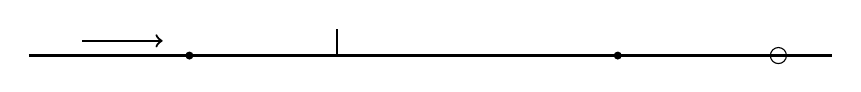
\begin{tikzpicture}[x=0.85cm,y=0.85cm]
\draw[thick] (0,0)--(12,0);
\draw[->,thick] (0.8,0.22)--(2.0,0.22);
\fill (2.4,0) circle (0.06);
\draw[thick] (4.6,0)--(4.6,0.40);
\fill (8.8,0) circle (0.06);
\draw (11.2,0) circle (0.12);
\end{tikzpicture}
\caption{Minimal redraw of the line analogy. The lecture only certifies a long line, directional arrows, and marked points, so the redraw is intentionally spare.}
\end{figure}

What matters in this picture is the distinction between local and global motion. Signals still move locally with a limiting speed relative to nearby points, but the total distance they must overcome can increase because more space is being inserted between source and destination.

\subsection{Question \& Answer}

\paragraph{How can a light signal fail to get back if nothing locally moves faster than light?}

Because the signal is not competing against the motion of a material object through a fixed background. It is competing against the growth of the distance itself. The signal always moves at the local limiting speed, but while it travels, the metric continues to expand. If the proper distance to the destination increases faster than the signal can reduce it, then the signal never returns. This is the key distinction between an expanding universe and an ordinary velocity-addition problem in special relativity.

The same analogy also explains cosmological redshift. A wave laid down on the expanding line stretches with the line. In the full theory this is not merely a picture; it is what one finds by solving a wave equation in an expanding geometry.

\section{Recap: Friedmann Equation and the Three Energy Components}

After the opening discussion Susskind resets the lecture and rewrites the basic expansion law. The central equation is
\begin{equation}
\left(\frac{\dot a}{a}\right)^2 = \frac{8\pi G}{3}\rho,
\qquad c=1.
\end{equation}
Here \(a(t)\) is the scale factor, \(\dot a / a\) is the Hubble parameter, and \(\rho\) is the total energy density.

\begin{figure}
\centering

\includegraphics[width=0.74\textwidth]{lecture_04_figure_03.png}
\caption{The basic expansion equation on the board, written beneath the line analogy. The cropped metric fragment on the right is only partial; the lecture's operative equation is the Friedmann equation shown clearly here.}
\end{figure}

\begin{figure}
\centering
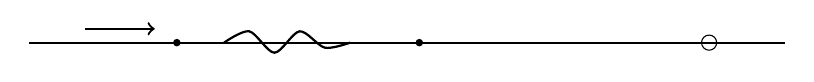
\begin{tikzpicture}[x=0.8cm,y=0.8cm]
\draw[thick] (0,0)--(12,0);
\draw[->,thick] (0.9,0.22)--(2.0,0.22);
\fill (2.35,0) circle (0.06);
\draw[thick] plot[smooth] coordinates {(3.1,0) (3.5,0.18) (3.9,-0.16) (4.3,0.18) (4.7,-0.08) (5.1,0)};
\fill (6.2,0) circle (0.06);
\draw (10.8,0) circle (0.12);
\end{tikzpicture}
\caption{Minimal redraw of the line sketch with a small disturbance, kept schematic because the board marks are analogical rather than fully labeled geometry.}
\end{figure}

The right-hand side can be built from several contributions. The lecture reviews three:
\begin{itemize}
\item matter, meaning objects approximately at rest in the comoving frame,
\item radiation, meaning photons and other effectively massless components,
\item vacuum energy, written as \(\rho_0\), which does not dilute as the universe expands.
\end{itemize}

For matter and radiation the familiar scaling laws had already been established in earlier lectures:
\begin{align}
\rho_m &\propto a^{-3},
&
a(t) &\propto t^{2/3},
\\
\rho_r &\propto a^{-4},
&
a(t) &\propto t^{1/2}.
\end{align}
For the third component Susskind begins by simply stating the essential fact:
\begin{equation}
\rho_0 = \text{constant}.
\end{equation}
That is the strange one, and the lecture spends the rest of its mathematics explaining why it corresponds to a very special equation of state.

\section{Pressure from Radiation and Matter}

The first technical job is to understand pressure. Radiation is the clean example, because its pressure can be built directly from momentum transfer.

\paragraph{One-dimensional photon box.}
Take a line segment of length \(L\), with photons bouncing between the two ends. A photon with momentum magnitude \(p\) reverses its momentum when it reflects, so the momentum change per collision is
\begin{equation}
\Delta p = 2p .
\end{equation}
The time between successive collisions with the same wall is
\begin{equation}
\Delta t = \frac{2L}{c},
\end{equation}
since the photon must go across the segment and come back. Therefore the average force on the wall is
\begin{equation}
F = \frac{\Delta p}{\Delta t} = \frac{pc}{L}.
\end{equation}
For a photon,
\begin{equation}
E = pc,
\end{equation}
so this becomes
\begin{equation}
F = \frac{E}{L}.
\end{equation}
In this one-dimensional toy model the energy density is energy per unit length, \(\rho = E/L\), so the result is
\begin{equation}
P=\rho
\end{equation}
with the understanding that here \(P\) is just force on the end of the interval and \(\rho\) means energy per unit length.

\begin{figure}
\centering
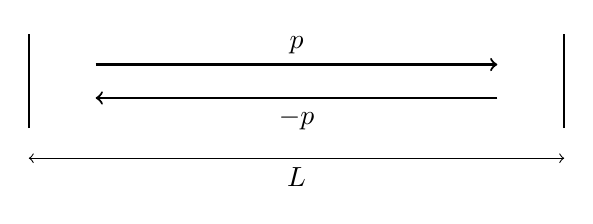
\begin{tikzpicture}[x=0.85cm,y=0.85cm]
\draw[thick] (0,0)--(0,1.4);
\draw[thick] (8,0)--(8,1.4);
\draw[<->] (0,-0.45)--(8,-0.45) node[midway,below]{$L$};
\draw[->,thick] (1,0.95)--(7,0.95) node[midway,above]{$p$};
\draw[->,thick] (7,0.45)--(1,0.45) node[midway,below]{$-p$};
\end{tikzpicture}
\caption{One-dimensional photon-in-a-box picture used in the radiation-pressure derivation. The wall receives momentum \(2p\) at each reflection.}
\end{figure}

\paragraph{Three dimensions.}
Now pass to a three-dimensional box. If all photons moved only along one axis, the same reasoning would give pressure on one pair of faces, but none on the others. That is not the physically relevant situation. In an isotropic radiation bath the momenta are distributed in all directions. The pressure on a given wall receives, on average, one third of the total energy density, because only one third of the kinetic content contributes to any given Cartesian direction. The result is
\begin{equation}
P_r = \frac{\rho_r}{3}.
\end{equation}

\begin{figure}
\centering
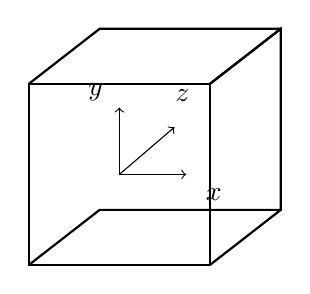
\begin{tikzpicture}[x=1cm,y=1cm]
\draw[thick] (0,0)--(2.3,0)--(2.3,2.3)--(0,2.3)--cycle;
\draw[thick] (0,0)--(0.9,0.7)--(3.2,0.7)--(3.2,3.0)--(2.3,2.3);
\draw[thick] (2.3,0)--(3.2,0.7);
\draw[thick] (2.3,2.3)--(3.2,3.0);
\draw[thick] (0,2.3)--(0.9,3.0)--(3.2,3.0);
\draw[->] (1.15,1.15)--(2.0,1.15);
\draw[->] (1.15,1.15)--(1.15,2.0);
\draw[->] (1.15,1.15)--(1.85,1.75);
\node at (2.35,0.9){$x$};
\node at (0.85,2.2){$y$};
\node at (1.95,2.15){$z$};
\end{tikzpicture}
\caption{Schematic three-dimensional box used to motivate isotropic radiation pressure. Each pressure component receives one third of the total energy density.}
\end{figure}

\paragraph{Cold matter.}
The matter-dominated case is the opposite limit. Consider a comoving box moving with the cosmological flow. Cold matter is approximately at rest relative to the box walls. It has energy density, since each particle contributes its rest energy, but it does not bang into the walls. Hence it exerts no pressure:
\begin{equation}
P_m = 0.
\end{equation}

\begin{figure}
\centering

\includegraphics[width=0.74\textwidth]{lecture_04_figure_04.png}
\caption{Board summary comparing matter and radiation after the pressure discussion. The row-by-row layout is itself part of the lecture's rhetoric.}
\end{figure}

The board comparison can be written cleanly as
\begin{align}
\text{matter:} \qquad & a(t)\sim t^{2/3}, \qquad P=0,
\\
\text{radiation:} \qquad & a(t)\sim t^{1/2}, \qquad P=\frac{\rho_r}{3}.
\end{align}

\section{Equation of State and Density Scaling}

Having two concrete examples in hand, Susskind now abstracts. The pressure is often proportional to the energy density:
\begin{equation}
P = w\rho .
\end{equation}
On the board he writes \(\omega\); we will use \(w\). The special cases already found are
\begin{equation}
w=0 \quad \text{for cold matter},
\qquad
w=\frac{1}{3} \quad \text{for radiation}.
\end{equation}
The point of introducing \(w\) is not jargon for its own sake. It is that once \(w\) is known, one can determine how the corresponding energy density changes as the universe expands.

\begin{figure}
\centering

\includegraphics[width=0.74\textwidth]{lecture_04_figure_05.png}
\caption{Board evidence for the equation-of-state parameter. Susskind points to \(P=\omega\rho\) as the conceptual center, while the density-scaling derivation is partially visible on the right.}
\end{figure}

\subsection{Question \& Answer}

\paragraph{Why should the pressure-to-density ratio determine how the density changes with the scale factor?}

Because expansion does work. The subtle point is that when a comoving box grows, the total energy inside it need not stay fixed. Some of that energy can be spent doing work on the walls. The larger the pressure, the more strongly the expansion changes the internal energy.

Take a comoving box of volume \(V\). If its walls move outward by an amount that changes the volume by \(dV\), then the work done by the contents on the walls is \(P\,dV\). Therefore the internal energy \(E\) of the box decreases by
\begin{equation}
dE = -P\,dV.
\end{equation}
But the total internal energy is
\begin{equation}
E = \rho V,
\end{equation}
so
\begin{equation}
dE = \rho\,dV + V\,d\rho.
\end{equation}
Equating the two expressions for \(dE\), we obtain
\begin{equation}
\rho\,dV + V\,d\rho = -P\,dV,
\end{equation}
or
\begin{equation}
V\,d\rho = -(\rho+P)\,dV.
\end{equation}
Now insert the equation of state \(P=w\rho\):
\begin{equation}
V\,d\rho = -(1+w)\rho\,dV.
\end{equation}
Divide by \(\rho V\):
\begin{equation}
\frac{d\rho}{\rho} = -(1+w)\frac{dV}{V}.
\end{equation}
Integrating,
\begin{equation}
\ln \rho = -(1+w)\ln V + \text{const},
\end{equation}
so
\begin{equation}
\rho \propto V^{-(1+w)}.
\end{equation}
For a comoving box one has \(V\propto a^3\), and therefore
\begin{equation}
\rho \propto a^{-3(1+w)}.
\end{equation}

This is the real payoff of the section. The equation-of-state parameter controls the dilution law.

As a check,
\begin{align}
w=0
&\Longrightarrow
\rho \propto a^{-3},
\\
w=\frac{1}{3}
&\Longrightarrow
\rho \propto a^{-4}.
\end{align}
These are exactly the matter and radiation laws with which the lecture began.

Once \(\rho(a)\) is known, one can return to Friedmann's equation and solve for \(a(t)\). For the cases already discussed, this reproduces the known expansion laws \(a\sim t^{2/3}\) and \(a\sim t^{1/2}\). The lecture does not insist on the general formula here. What matters is the structure: \(w\) determines how \(\rho\) changes, and that in turn determines how the universe expands.

\section{Vacuum Energy as the Special Case \(w=-1\)}

Now the exceptional case emerges. If
\begin{equation}
w=-1,
\end{equation}
then
\begin{equation}
P=-\rho
\end{equation}
and the general scaling law gives
\begin{equation}
\rho \propto a^{-3(1+w)} = a^0 = \text{constant}.
\end{equation}
This is precisely the behavior of vacuum energy. Denote it by \(\rho_0\):
\begin{equation}
\rho=\rho_0=\text{const}.
\end{equation}

\subsection{Question \& Answer}

\paragraph{How can positive energy density come with negative pressure, and why does that not make the theory inconsistent?}

Because negative pressure is just tension. Positive pressure pushes outward on the walls of a box. Negative pressure pulls inward, the way a stretched rubber band pulls its ends together. There is nothing mathematically inconsistent about this. The energy density remains positive; only the pressure changes sign. In the lecture this is exactly how the mystery is deflated: negative pressure is not an absurdity, it is an ordinary physical notion with the opposite sign convention.

Insert the constant density \(\rho_0\) into Friedmann's equation:
\begin{equation}
\left(\frac{\dot a}{a}\right)^2 = \frac{8\pi G}{3}\rho_0.
\end{equation}
The right-hand side is now just a constant. Define
\begin{equation}
H=\sqrt{\frac{8\pi G\rho_0}{3}}.
\end{equation}
Then
\begin{equation}
\frac{\dot a}{a}=H,
\qquad\text{so}\qquad
\dot a = Ha.
\end{equation}
This differential equation has the exponential solution
\begin{equation}
a(t)=a_{\ast}\exp(Ht)
=
a_{\ast}\exp\!\left(\sqrt{\frac{8\pi G\rho_0}{3}}\,t\right).
\end{equation}

That is why vacuum domination gives accelerated expansion. The scale factor does not merely keep increasing; its rate of increase is proportional to itself.

At this point Susskind remarks that one often packages the vacuum energy into the cosmological constant \(\Lambda\). The lecture treats the normalization as historically conventional and slightly messy. For the present discussion it is cleaner to keep speaking in terms of \(\rho_0\): the vacuum energy density. The physics is the constancy of \(\rho_0\), not the bookkeeping of factors of \(3\).

There is, as always, a second sign when one takes the square root. The equations permit both expanding and contracting branches. In these notes, as in the lecture, we follow the expanding branch.

\section{Cosmic Eras, Observational Reconstruction, and the Late-Time Horizon}

Once the general framework is in place, the lecture zooms back out. The universe passes through three broad eras:
\begin{itemize}
\item an early radiation-dominated era,
\item an intermediate matter-dominated era,
\item a late vacuum-dominated era.
\end{itemize}
The reason is simple. Radiation falls off fastest, matter less fast, and vacuum energy not at all:
\begin{align}
\rho_r &\propto a^{-4},
&
\rho_m &\propto a^{-3},
&
\rho_0 &= \text{const}.
\end{align}

\begin{figure}
\centering
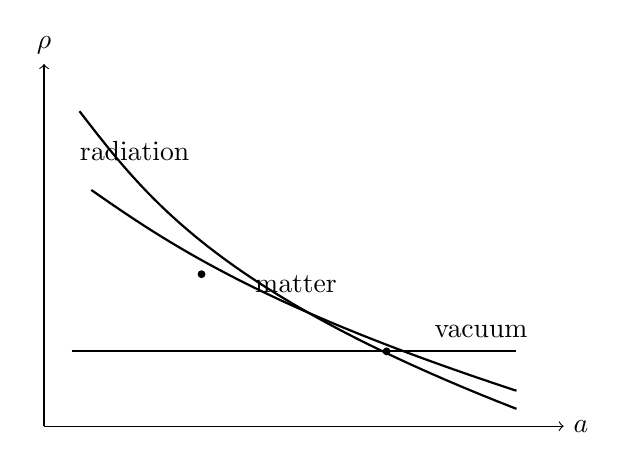
\begin{tikzpicture}[x=1cm,y=1cm]
\draw[->] (0,0)--(6.6,0) node[right]{$a$};
\draw[->] (0,0)--(0,4.6) node[above]{$\rho$};
\draw[thick] (0.45,4.0) .. controls (1.3,2.9) and (2.2,1.7) .. (6.0,0.22);
\draw[thick] (0.6,3.0) .. controls (1.6,2.3) and (2.8,1.5) .. (6.0,0.45);
\draw[thick] (0.35,0.95)--(6.0,0.95);
\fill (2.0,1.93) circle (0.05);
\fill (4.35,0.95) circle (0.05);
\node at (1.15,3.5) {radiation};
\node at (3.2,1.8) {matter};
\node at (5.55,1.2) {vacuum};
\end{tikzpicture}
\caption{Qualitative energy-density history as a function of scale factor. Radiation dominates at small \(a\), matter at intermediate \(a\), and vacuum at large \(a\).}
\end{figure}

The corresponding history of the scale factor is therefore qualitative rather than mysterious:
\begin{itemize}
\item early on, \(a(t)\sim t^{1/2}\),
\item then \(a(t)\sim t^{2/3}\),
\item later, \(a(t)\) bends upward toward exponential growth.
\end{itemize}

\begin{figure}
\centering
\begin{tikzpicture}[x=1cm,y=1cm]
\draw[->] (0,0)--(6.6,0) node[right]{$t$};
\draw[->] (0,0)--(0,4.6) node[above]{$a(t)$};
\draw[thick] (0.35,0.25) .. controls (1.0,1.0) and (1.7,1.6) .. (2.25,2.0);
\draw[thick] (2.25,2.0) .. controls (3.2,2.55) and (4.0,3.0) .. (4.65,3.3);
\draw[thick] (4.65,3.3) .. controls (5.1,3.45) and (5.55,3.8) .. (6.15,4.5);
\node at (1.1,1.55) {$t^{1/2}$};
\node at (3.45,2.75) {$t^{2/3}$};
\node at (5.45,4.05) {exponential};
\end{tikzpicture}
\caption{Qualitative time history of the scale factor: radiation era, matter era, then accelerated expansion.}
\end{figure}

How do we know this history? We do not see the future, but we do see the past. Looking farther out means looking earlier. By measuring distances and recession speeds for galaxies at different lookback times, one reconstructs the evolution of the Hubble parameter and therefore the curve \(a(t)\). According to the lecture, the evidence strongly supports a transition from matter domination to a late phase that is very close to cosmological-constant domination.

At late times, when vacuum energy dominates, the Hubble parameter becomes asymptotically constant:
\begin{equation}
H=\sqrt{\frac{8\pi G\rho_0}{3}}.
\end{equation}
Then the horizon distance is determined by the condition \(Hd_H=1\), so
\begin{equation}
d_H=\frac{1}{H}=\frac{1}{\sqrt{8\pi G\rho_0/3}}.
\end{equation}
The striking point is that this horizon distance is fixed once pure exponential expansion sets in. Galaxies continue to move outward and eventually pass beyond this fixed horizon, becoming more and more redshifted until they disappear from view.

The lecture briefly restores the curvature term that had been omitted for most of the discussion:
\begin{equation}
\left(\frac{\dot a}{a}\right)^2
=
\frac{8\pi G}{3}\rho
-
\frac{K}{a^2}.
\end{equation}
Historically this term supported the old Big-Crunch picture: a universe that expands for a while and then recontracts. The modern point of view in the lecture is different. Empirically \(K\) appears to be very small, while vacuum energy drives the late accelerated expansion. So the old closed-and-crunching picture is mathematically possible, but not the one suggested by current evidence.

For the lecture-era present-day composition one may quote the approximate fractions
\begin{align}
\frac{\rho_0}{\rho_{\text{total}}} &\sim 0.7,
&
\frac{\rho_m}{\rho_{\text{total}}} &\sim 0.3,
\\
\frac{\rho_{\text{lum}}}{\rho_{\text{total}}} &\sim 0.05,
&
\frac{\rho_{\text{dark}}}{\rho_{\text{total}}} &\sim 0.25,
\end{align}
with radiation negligible compared with matter and vacuum energy. Because dark matter and luminous matter both scale as \(a^{-3}\), their ratio stays roughly fixed even while the total cosmic balance shifts from one era to another.

The lecture ends by turning toward the next question: geometry. If one knows the distance to the surface of last scattering and has good reason to assign a physical size to the largest visible lumps there, then the observed angular size tests spatial curvature. A flat geometry gives the Euclidean angle; positive or negative curvature shifts it.

\begin{figure}
\centering
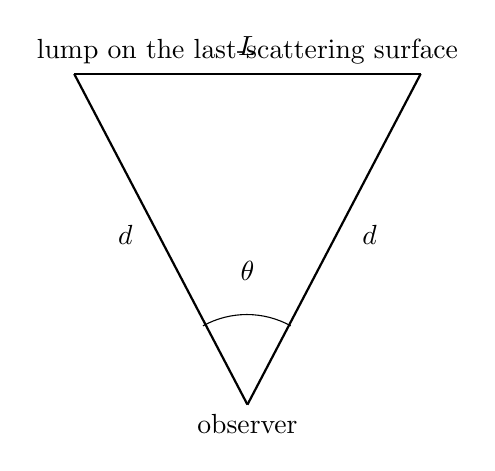
\begin{tikzpicture}[x=1cm,y=1cm]
\coordinate (O) at (0,0);
\coordinate (L) at (-2.2,4.2);
\coordinate (R) at (2.2,4.2);
\draw[thick] (O)--(L);
\draw[thick] (O)--(R);
\draw[thick] (L)--(R);
\draw (0.55,1.0) arc[start angle=61,end angle=119,radius=1.15];
\node at (0,1.7) {$\theta$};
\node at (0,4.55) {$L$};
\node at (-1.55,2.15) {$d$};
\node at (1.55,2.15) {$d$};
\node[below] at (O) {observer};
\node[above] at (0,4.2) {lump on the last-scattering surface};
\end{tikzpicture}
\caption{Preview of the next lecture's geometry test: the observed angle subtended by a standard lump on the last-scattering surface probes spatial curvature.}
\end{figure}

This closing geometry argument is only a setup here. The real accomplishment of the present lecture is earlier: pressure has been tied to energy density, \(w\) has been introduced as the useful organizing parameter, and vacuum energy has emerged as the special case \(w=-1\).

\section{Summary}

The lecture begins with questions about the microwave background and ends with the global fate of the universe, but the mathematical spine in the middle is quite tight. Radiation pressure gives \(P=\rho/3\), cold matter gives \(P=0\), and both are unified by
\begin{equation}
P=w\rho .
\end{equation}
Thermodynamics then turns this into the density-scaling law
\begin{equation}
\rho\propto a^{-3(1+w)}.
\end{equation}
The special value \(w=-1\) corresponds to vacuum energy, constant \(\rho_0\), negative pressure, and exponential expansion. From there the late-time horizon, the three cosmic eras, and the observational reconstruction of the expansion history all follow in a clean sequence.